\chapter{空間全体を対象とした幾何音響解析}

\section{幾何音響解析手法について}
幾何音響解析手法とは、音の波動としての性質を無視して、その伝搬を幾何的に取り扱う手法のことである$^{\text{\cite{02-5}}}$。非常に直感的で理解しやすい方法であり、あまり多くの計算機資源を必要とせず、計算時間も波動音響解析手法と比べ短いため、大規模空間を扱う際の現実的手法として広く用いられている。厳密な予測が必要となる詳細設計の段階では音響縮尺模型実験や波動音響解析に頼らざるを得ないが、基本計画段階における検討や初期反射音構造の予測等に対しては大変有用であると考えられている。
幾何音響学に基づいた代表的なコンピュータシミュレーション手法として、音線法と鏡像法が挙げられる(\figref{音線法と鏡像法})。
\\ 音線法(Ray-tracing method)とは、音源から等立体間隔で多数の音線を出すことで、反射伝搬経路を追跡計算する手法であり、距離減衰は音線間の広がり(音線の密度)によって考慮される。なお、有限の間隔で放射された音線が丁度受音点を通過することは極めて稀なため、有限の大きさを持つ受音領域を設けることが一般的である。しかしながら、受音点が領域を持つゆえに同一経路の反射音が重複したり、現実にはない反射経路を抽出したり等の計算誤差が生じる。この問題を解決するため、複数のアルゴリズムが考案されている$^{\text{\cite{02-6}}}$。
\\ 鏡像法(Image source method)は周壁各面における音源の鏡像を幾何学的に求め、各鏡像から受音点までの経路を求める手法である。距離減衰と通った反射面の吸音率からインパルス応答を近似的に求めることができるが、反射次数の増加とともに鏡像の数が指数関数的に増加するため、高次の反射音まで求めることは困難である$^{\text{\cite{02-5}}}$。
\\ 音線法と鏡像法のいずれも、初期反射音の検討に対して非常に有用であると考えられるが、拡散反射を考慮できない幾何音響シミュレーションのみでは、反射回数が増加するに従い、現実の音場との誤差が大きくなってしまう。そこで近年では乱反射率(Scattering coefficient)などの導入により、室内音場の長時間のインパルス応答を求めようとする試みがある。
\begin{figure}[H]
    \centering
    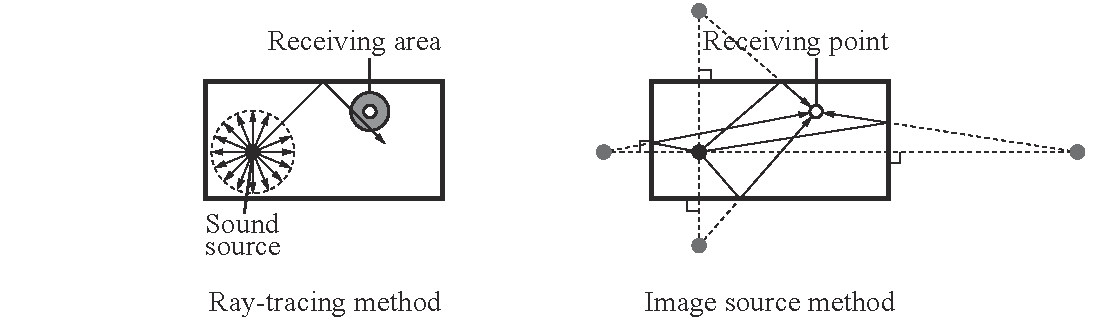
\includegraphics[keepaspectratio,scale=0.65]{02_att/kikaonkyo.pdf}
    \caption{\hspace{1mm}Concepts of ray-tracing method and image source method}
    \label{fig:音線法と鏡像法}
\end{figure}

\section{解析条件}
本研究で用いる幾何音響解析ソフトには3つの解析タイプ(Audio area mapping, Early part detailed, Full detailed calculation)があり、それぞれ音線法、鏡像法、Randomized Tail-corrected Cone-tracing method (RTC)により計算される(\tabref{3つの解析タイプ})。
RTCとは音線の先に円の有限領域をもたせるCone-tracingと標準的な音線法及び鏡像法をハイブリッドした解析手法である。
\\ 本研究ではこれらのうち、後期反射音までのインパルス応答を算出するFull detailed calculationから室内音響物理指標を、9次反射音までのインパルス応答(方向情報含む)(\figref{Early_IR})を算出するEarly part detailedから方向別物理量を各々求めた。解析条件を解析タイプ別に\tabref{Full_set}と\tabref{Early_set}に示す。
\\
% 3つの解析手法について
\begin{table}[htbp]
\centering
\caption{Analysis methods and output data}
\label{tab:3つの解析タイプ}
\resizebox{\textwidth}{!}{%
\begin{tabular}{ccccc}
\Hline
Type & Prediction methods & \multicolumn{3}{c}{Output data} \\ \cline{3-5} 
 &  & \multicolumn{2}{c}{Impulse response} & Room acoustic parameters \\ \cline{3-4}
 &  & \multicolumn{1}{c|}{Time domain} & Spatial data &  \\ \hline
Audio area mapping & Ray-tracing method & $\times$ & $\times$ & $\bigcirc$ \\
Early part detailed & Image source method & Early part only & $\bigcirc$ & $\times$ \\
Full detailed calculation & RTC method & Full & $\bigtriangleup^{*}$ & $\bigcirc$ \\ \Hline
\multicolumn{5}{l}{$^{*}$ : limited spatial data}
\end{tabular}%
}
\end{table}

\begin{figure}[htbp]
    \centering
    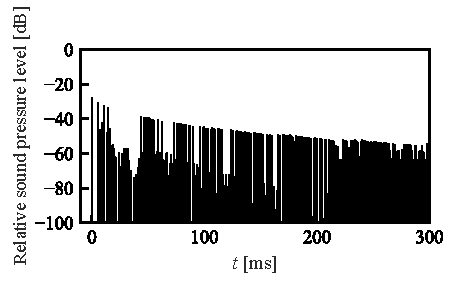
\includegraphics[keepaspectratio,scale=1]{02_att/Early_IR.pdf}
    \caption{\hspace{1mm}Impulse response calculated by Early part detailed}
    \label{fig:Early_IR}
\end{figure}

%EarlyとFullの解析条件
\begin{table}[htbp]
\begin{minipage}[t]{.45\textwidth}
    \begin{center}
    \caption{\hspace{1mm}Analysis conditions of Full detailed calculation}
    \label{tab:Full_set}
      \begin{tabular}{lc}%ひだり
      \Hline
      \multicolumn{1}{c}{Setting items} & Input value \\ \hline
      Number of rays & 99,9999 \\
      Truncation time [ms] & 3,500 \\ \Hline
      \end{tabular}
    \end{center}
  \end{minipage}
  %
  \hfill
  %
  \begin{minipage}[t]{.45\textwidth}
    \begin{center}
    \caption{\hspace{1mm}Analysis conditions of Early part detailed}
    \label{tab:Early_set}
      \begin{tabular}{lc}%みぎ
      \Hline
      \multicolumn{1}{c}{Setting items} & \multicolumn{1}{c}{Input value} \\ \hline
      Specular reflection order (0-9) & 9 \\
      Diffuse reflection order (0-1) & 1 \\
      Truncation time [ms] & 300 \\ \Hline
      \end{tabular}
    \end{center}
  \end{minipage}
\end{table}

\pagebreak
また、音速と空気吸収は\textbf{式}\ref{eq:speed_of_sound}と\textbf{式}\ref{eq:air_absorption}により定められる。本研究では一般的な室内を想定し、$\theta$=20[{\kern-.2em\r{}\kern-.3em C}]、$\phi=50[\%]$とした。すなわち、$c=343$[m/s]、 $m_b=0.63\times10^{-3}$[m$^{-1}$](500Hz)の条件下で解析を行った。

\begin{equation}
 \label{eq:speed_of_sound}
c = 331.4\sqrt{1+\frac{\theta}{273}}
\end{equation}
\begin{equation}
 \label{eq:air_absorption}
m_b = \mathrm{from \; ISO \; 9613.1^{\text{\cite{organizacion1993iso}}} \; based \; on \; \theta, \; f_b, \; and \; \phi}
\end{equation}
\hspace{2cm}$\theta$ : air temperature, {\kern-.2em\r{}\kern-.3em C}\\
\hspace{2cm}$m_b$ : air dissipation coefficient, m$^{-1}$\\
\hspace{2cm}$f_b$ : octave-band center frequency, Hz\\
\hspace{2cm}$\phi$ : relative humidity, $\%$

\section{解析モデル}
解析モデルは収容人員1,500人程度のコンサートホールを想定し、平面形状が矩形のモデル(TypeA)と扇形のモデル(TypeB)の2種類の空間モデルを対象とした。両モデルとも舞台高さを1m、奥行きを10mに統一した。
\\ 観測点は客席床面上と上部空間の音場性能を比較するために2m\(\times\)2m\(\times\)2mの格子状に(A)矩形モデルで840点、(B)扇形モデルで712点設けた。
また、音線が音源方向から到来したときに反射音到来角度が\(0^\circ\)になるよう、観測点の座標系を設定した。
音源は無指向性音源を舞台中央に高さ1.5mとした。両ホールの音響諸元を\tabref{解析モデルの音響諸元}に示す。
%%%%%%%%%%%%%%%%%%%
\begin{table}[htbp]
\centering
\caption{\hspace{1mm}Outlines of each type model}
\label{tab:解析モデルの音響諸元}
\begin{tabular}{lccccc}
\Hline
\multicolumn{1}{c}{Type} & \textit{V}{[}m$^3${]} & \textit{V}/\textit{S}{[}m{]} & \textit{RT}$^{*1}${[}s{]} &$\bar{\alpha}$& N$^{*2}$ \\ \hline
(A)Rectanglular shape & 15,268 & 3.8 & 2.2 & 0.24 & 840 \\
(B)Fan-shape & 15,329 & 3.8 & 2.2 & 0.24 & 712 \\ \Hline
\multicolumn{6}{l}{$^{*1}$ : calculated with Eyring-Knudsen formula (500Hz)} \\
\multicolumn{4}{l}{$^{*2}$ : N indicates the number of receiving points}
\end{tabular}
\end{table}
%%%%%%%%%%%%%%%%%%%

\subsection{形状の設計}
現存するホールを参考$^{\text{\cite{02-1}}}$に(A)矩形モデル及び(B)扇形モデルの設計を行った。
両ホールの断面図及び平面図を\figref{(A)矩形モデル及び(B)扇形モデル断面図}と\figref{(A)矩形モデル及び(B)扇形モデル平面図}に示す。

\newpage
%-------------------------------------------------------------------------
\begin{figure}[H]
    \centering
    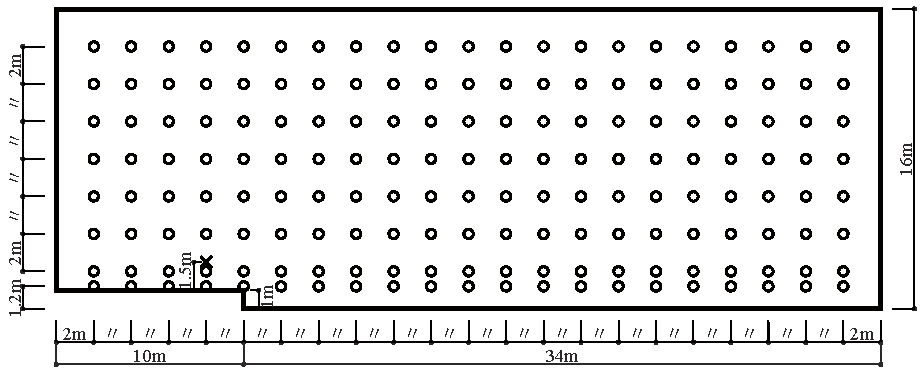
\includegraphics[keepaspectratio,scale=0.99]{02_att/rec_fan_zumen_1.pdf}
    \caption{\hspace{1mm}Section of rectangular shape and fan-shape}
    \label{fig:(A)矩形モデル及び(B)扇形モデル断面図}
\end{figure}

\begin{figure}[H]
    \centering
    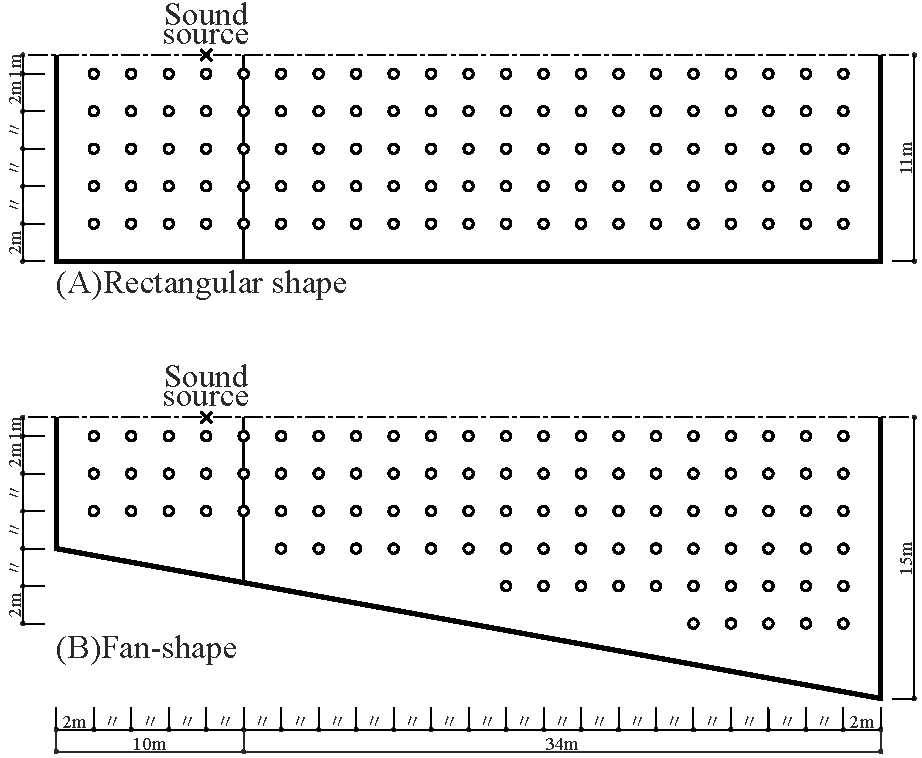
\includegraphics[keepaspectratio,scale=0.99]{02_att/rec_fan_zumen_2.pdf}
    \caption{\hspace{1mm}Plan of rectangular shape and fan-shape}
    \label{fig:(A)矩形モデル及び(B)扇形モデル平面図}
\end{figure}

\subsection{吸音率の設定}
室の内装面は客席床と後壁を吸音性、その他の面を反射性とし、両ホールの残響時間が等しくなるように現実的な吸音率(250$\sim$2kHz)$^{\text{\cite{01-3}\cite{02-1}\cite{02-2}}}$を設定した。客席床の吸音率については国内の標準的な1席(人+モケット張り椅子)の吸音力$^{\text{\cite{02-4}}}$を1席あたりの床面積(=0.6m$^2$)で除した値(\tabref{客席面の吸音率})を用いた。解析モデルに用いた吸音率を\tabref{解析モデルの吸音率}に示す。
\\
\\
%%%%%%%%%%%%%%%%%%%
\begin{table}[htbp]
\begin{center}
\caption{\hspace{1mm}Sound absorption and sound absorption coefficient of seating area}
\label{tab:客席面の吸音率}
\begin{tabular}{llcccccc}
\Hline
&&\multicolumn{6}{c}{Frequency{[}Hz{]}}\\\cline{3-8}
&&125&250&500&1k&2k&4k\\\hline
(a)&\begin{tabular}[c]{@{}l@{}}Sound absorption of a seat \\(human and moquette-clad chair) \end{tabular}&0.23&0.32&0.40&0.43&0.43&0.41\\\hline
(b)&\begin{tabular}[c]{@{}l@{}}Sound absorption coefficient \\equivalent to (a)\end{tabular}&0.38&0.53&0.67&0.72&0.72&0.68\\\Hline
\end{tabular}
\end{center}
\end{table}
%%%%%%%%%%%%%%%%%%%
\\
\\
%%%%%%%%%%%%%%%%%%%
\begin{table}[htbp]
\centering
\caption{\hspace{1mm}Sound absorption coefficient of models}
\label{tab:解析モデルの吸音率}
\resizebox{\textwidth}{!}{%
\begin{tabular}{llcccccc}
\Hline
                         &                                           & \multicolumn{6}{c}{Frequency{[}Hz{]}}   \\ \cline{3-8} 
\multicolumn{1}{c}{Site} & \multicolumn{1}{c}{Material}              & 125  & 250  & 500  & 1k   & 2k   & 4k   \\ \hline
Ceiling \_ main floor    & Plaster board (12mm) with large air space & 0.25 & 0.15 & 0.10 & 0.08 & 0.06 & 0.05 \\
Ceiling \_ stage         & Acoustic reflector                        & 0.15 & 0.15 & 0.10 & 0.08 & 0.07 & 0.06 \\
Floor \_ main floor      & Human and moquette-clad chair             & 0.38 & 0.53 & 0.67 & 0.72 & 0.72 & 0.68 \\
Floor \_ stage           & Floor joist of stage (45mm)               & 0.15 & 0.10 & 0.08 & 0.07 & 0.05 & 0.05 \\
Side wall \_ main floor  & Concrete                                  & 0.01 & 0.02 & 0.02 & 0.03 & 0.03 & 0.03 \\
Rear wall \_ main floor  & Glass wool (25mm) with large air space    & 0.55 & 0.80 & 0.75 & 0.48 & 0.33 & 0.15 \\
Wall \_ stage            & Acoustic reflector                        & 0.15 & 0.15 & 0.10 & 0.08 & 0.07 & 0.06 \\ \Hline
\end{tabular}%
}
\end{table}
%%%%%%%%%%%%%%%%%%%
\pagebreak
\subsection{乱反射率の設定}
乱反射率(Scattering coefficient)はISO17497-1$^{\text{\cite{iso2004acoustics}}}$の中で壁面の全反射エネルギーに対する鏡面反射成分以外のエネルギーの割合として定義され、\textbf{式}\ref{eq:scatter}で表される。ここで$E_{total}$は全反射エネルギー、$E_{spec}$は鏡面反射エネルギーである。

\begin{equation}
 \label{eq:scatter}
s_{\theta}=1-\frac{E_{spec}}{E_{total}}
\end{equation}

\vspace{0.8cm}

解析では、周波数に応じて座席部に0.3$\sim$0.7を、それ以外の面に0.1を与えた$^{\text{\cite{02-3}}}$。
解析モデルに用いた乱反射率を\tabref{解析モデルの乱反射率}に示す。\\
 また、壁面隅角部における音の散乱(端部散乱)を考慮した乱反射率を与える研究$^{\text{\cite{02-7}}}$が進められている。
壁面端部から$\lambda$/8分の面積を1、それ以外の面積を0として面積平均した乱反射率を吸音面の接合面に与えたときに実測との対応が良くなることが既往の研究$^{\text{\cite{02-8}}}$から明らかになっているが、これは本研究で使用する幾何音響解析ソフトの端部散乱を考慮した乱反射率(壁面端部から$\lambda$/4分の面積を0.5、それ以外の面積を0として面積平均したもの(\textbf{式}\ref{eq:付加乱反射率計算式}、\figref{壁面端部}))に近似する。
解析モデルにおいて端部散乱を考慮した面を\tabref{端部散乱を適用する面}に示す。

\vspace{0.8cm}

%%%%%%%%%%%%%%%%%%%
\begin{table}[htbp]
\centering
\caption{\hspace{1mm}Scattering coefficient of models}
\label{tab:解析モデルの乱反射率}
\resizebox{\textwidth}{!}{%
\begin{tabular}{llcccccc}
\Hline
&& \multicolumn{6}{c}{Frequency{[}Hz{]}}   \\ \cline{3-8} 
\multicolumn{1}{c}{Site} & \multicolumn{1}{c}{Material}              & 125  & 250  & 500  & 1k   & 2k   & 4k   \\ \hline
Ceiling \_ main floor    & Plaster board (12mm) with large air space & 0.10 & 0.10 & 0.10 & 0.10 & 0.10 & 0.10 \\
Ceiling \_ stage         & Acoustic reflector                        & 0.10 & 0.10 & 0.10 & 0.10 & 0.10 & 0.10 \\
Floor \_ main floor      & Human and moquette-clad chair             & 0.30 & 0.40 & 0.50 & 0.60 & 0.70 & 0.80 \\
Floor \_ stage           & Floor joist of stage (45mm)               & 0.10 & 0.10 & 0.10 & 0.10 & 0.10 & 0.10 \\
Side wall \_ main floor  & Concrete                                  & 0.10 & 0.10 & 0.10 & 0.10 & 0.10 & 0.10 \\
Rear wall \_ main floor  & Glass wool (25mm) with large air space    & 0.10 & 0.10 & 0.10 & 0.10 & 0.10 & 0.10 \\
Wall \_ stage            & Acoustic reflector                        & 0.10 & 0.10 & 0.10 & 0.10 & 0.10 & 0.10 \\ \Hline
\end{tabular}%
}
\end{table}
%%%%%%%%%%%%%%%%%%%

\vspace{0.8cm}

\begin{table}[htbp]
\begin{equation}
 \label{eq:付加乱反射率計算式}
 s_{\scalebox{0.5}{effective}} = s_{\scalebox{0.5}{surface}} + \frac{s_{\scalebox{0.5}{edge}}
 S_{\scalebox{0.5}{edge}}}{S_{\scalebox{0.5}{surface}}}\\
\end{equation}
\hspace{2cm}$s_{\scalebox{0.5}{edge}} = 0.5$\\
\hspace{2cm}$s_{\scalebox{0.5}{surface}}$ : The normal surface scattering coefficient\\
\hspace{2cm}$S_{\scalebox{0.5}{edge}}$ : The area of an edge quarter of a wavelength wide\\
\hspace{2cm}$S_{\scalebox{0.5}{surface}}$ : The complete plane or sub-plane area\\
\end{table}

\begin{figure}[htbp]
    \centering
    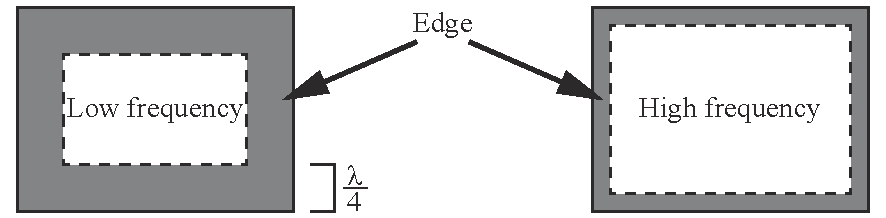
\includegraphics[keepaspectratio,scale=0.8]{02_att/edge.pdf}
    \caption{\hspace{1mm}Area of $\lambda$/4 from wall end}
    \label{fig:壁面端部}
\end{figure}

%%%%%%%%%%%%%%%%%%%
\begin{table}[htbp]
\centering
\caption{\hspace{1mm}The surface which apply to edge diffusion}
\label{tab:端部散乱を適用する面}
\begin{tabular}{llc}
\Hline
\multicolumn{1}{c}{Site} & \multicolumn{1}{c}{Type} & Apply edge diffusion to surface \\ \hline
Ceiling \_ main floor    & Reflective               & *                               \\
Ceiling \_ stage         & Reflective               & *                               \\
Floor \_ main floor      & Absorptive               &                                 \\
Floor \_ stage           & Reflective               & *                               \\
Side wall \_ main floor  & Reflective               & *                               \\
Rear wall \_ main floor  & Absorptive               &                                 \\
Wall \_ stage            & Reflective               & *                               \\ \Hline
\end{tabular}
\end{table}
%%%%%%%%%%%%%%%%%%%
